
\chapter{Evaluation}
\label{sec:Evaluation}
This chapter describes and illustrates the experiments performed on the system. In the chapter, section \ref{sec:ExperimentsSetup} describes the experimental setup. Section \ref{sec:Datasets} describes the datasets used. Section \ref{sec:ResultsDetails} demonstrates and analyzes the results. 

The system has two main parts the DPSO stroke segmentation and symbol recognition. Each part is evaluated separately. The preprocessing procedures and computation is evaluated using their effect on the segmentation algorithm. These results are reported in section \ref{sec:ResultsDetails}. The effect of number of agents, the error thresholds and various other PSO parameters are investigated in Section \ref{sec:PSO}. %The results presented in Section \ref{sec:ResultsDetails} and \ref{sec:PSO}.  

The recognition system evaluation is presented in Section \ref{sec:SegmentationAlgorithms}. The recognition rate (computed as the number of correctly recognized samples divided by the total number of samples in the test) for each segmentation algorithm compared to another segmentation algorithm are reported in \ref{sec:recognitionAlgorithms}. Next, a comparison between different shapes and datasets and it influence on the recognition rate is presented in Section \ref{sec:EffectsofSymbolComplixity}. Finally, a comparison between different feature vectors is reported in Section \ref{sec:featuresComparisions}.

\section{Datasets}
\label{sec:Datasets}
Three different data set were used, table \ref{tab:datasets} shows a comparison between the three datasets used in our experiments. 

%For classifier and algorithm testing the system used a data set collected by
\begin{description}
	\item [Hse Dataset] (denoted as Hs-DB) Data set collected by \cite{HeloiseBeautification} and was previously used by \cite{Oltmans07} as benchmark for sketch recognition problem. The data are drawn by 16 users each of them have drawn from 50 to 60 samples for each shape. Figure \ref{fig:symbolSet} shows the shapes used in the data set. The dataset was divided into 75\% training set and 25\% test set. Five different splits for the training and test data are generated from the dataset. In worth noting that \cite{HeloiseBeautification} and \cite{Oltmans07} achieved 96.7\% and  94.4\%  on this dataset respectively. %, 94.4\%  , which
%is comparable to the 96.7%  %The results displayed are the average recognition accuracy of the four splits resulted from the classifier after recognizing the symbols.
		\item [Multi Domain Dataset] (denoted as MD-DB) A dataset we collected manually from different users. The dataset contains symbols from two different domains Electrical Engineering symbols (EL-DB) and logic design symbols (LD-DB). Data are collected from 7 different users each of them have drawn from 20 to 40 samples of each shapes. Figures \ref{fig:LogicSet} and \ref{fig:ElectSet} show some of the shapes used in the dataset. Symbols from different domains were gathered to evaluate the system throughout different types of shapes. Users were requested to draw symbols without any restriction on style, size or orientations. The dataset was divided into 75\% training set and 25\% test set. Five different splits for the training and test data are generated from the dataset. %In worth noting that \cite{Oltmans07} gathered similar dataset and achieved 89\% on it   %The results displayed are the average recognition accuracy of the four splits resulted from the classifier after recognizing the symbols. 
\end{description}

 %We divided the dataset equally into training set and test set.  The results displayed are the recognition accuracy resulted from the classifier after recognizing the symbols. \\
%We divided the dataset into four sets each set contains four different users. Furthermore, each set is divided into train and test set where the trained set where used to train the classifiers and the test set where used for testing.  The algorithms are then tested using the four sets and the results are averaged.
\begin{figure}[]\centering
\fbox{  \parbox{8cm}{% 
		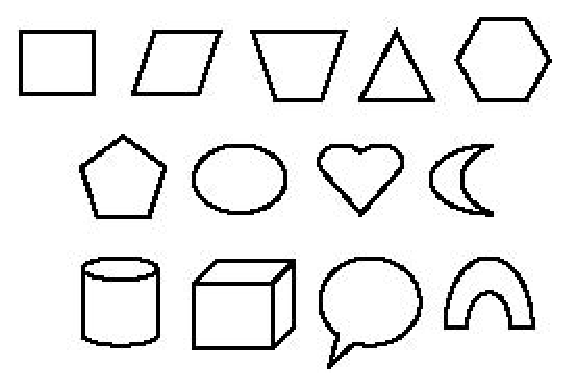
\includegraphics[scale=0.7]{images/symbolSet.eps}	}
		}
	\caption{The Symbol Set}
	\label{fig:symbolSet}
\end{figure}

\begin{figure}[]\centering

		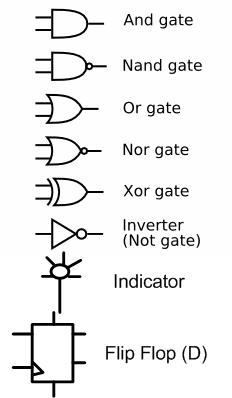
\includegraphics[scale=0.9]{paperImages/logicSet.jpg.eps}	

	\caption{Example of Logic Symbols}
	\label{fig:LogicSet}
\end{figure}
\begin{figure}[]\centering

		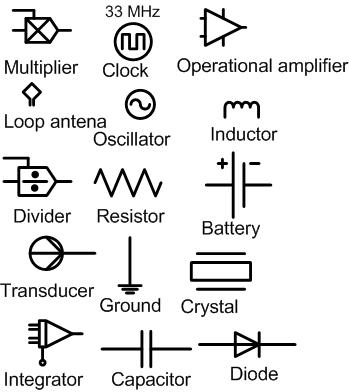
\includegraphics[scale=0.9]{paperImages/EelectImage.jpg.eps}	

	\caption{Example of Electrical Symbols}
	\label{fig:ElectSet}
\end{figure}
\begin{table}
\begin{center}
\scalebox{0.9}{
 \begin{tabular}{|p{5cm}|p{2.5cm}|p{2.5cm}|p{2.5cm}|}
 \hline
 & Hs-DB &  EL-DB & LD-DB \\ \hline
No of samples  &  7791 & 2764 & 1859 \\ \hline
No of categories  & 13 & 15 & 8 \\ \hline
Avg. Samples per Category& 600 & 184 & 232 \\\hline 
No of users  & 16 & 7 & 7 \\  \hline
Balanced & Yes&No & No \\ \hline
Splits  & 5 random splits  & 5 random splits  & 5 random splits  \\ \hline
Examples & Figure \ref{fig:symbolSet}  & Figure \ref{fig:ELsymbolSet}  & Figure \ref{fig:LogicsymbolSet}   \\ \hline
\end{tabular}
}
\caption[Datasets Comparisons]{Datasets Comparisons} 
\label{tab:datasets}

\end{center}
\end{table}


%\section{Evaluations techniques}
%\label{sec:EvaluationsTechniques}
%\section {Curvature estimation results}
%\label{sec:Curvatureestimationresults}
\section{Performance Measures }
\label{sec:PerformanceMeasures}

\begin{description}
	\item[Segmentation Error] The segmentation error is computed from each stroke after segmentation as computed in Section \ref{sec:bestFit}. The error represents the sum of Square Root Error of the length from the point on the stroke to the estimated curve or line. 
	  
	\item [Recognition accuracy] We measure recognition performance for each algorithm by determining the number of correctly identified symbols in the whole dataset. Note that All the results are shown as the average of the four split of the dataset used. 
\end{description}

 

\section{Results}
\label{sec:ResultsDetails}

\subsection{PSO Algorithm}
\label{sec:PSO}

%Figure \ref{fig:SegErrPreCal} shows the \textit{Average Segmentation Error} using different preliminary calculation (Section \ref{sec:CurvatureCalculation}). The figure shows that using all computations (time difference, direction, speed and curvature) for each stroke decrease the Segmentation error. Figure \ref{fig:PossibledpPreCalculation} shows the average number of Possible dominant point $P_{pd}$ with respect to information used in the system. The results shows that the using all information increases the number of Possible dominate point $P_{pd}$ which in segmentation stage decreases the \textit{Segmentation Error}. It is worth noting that when using all information the number of Possible dominant point $P_{pd}$ is not the same as the sum of using every information alone. This is because we found out that there was some redundant points found using more than one information source.  


   
%\begin{figure}
%	\centering
%		\includegraphics[scale=0.5]{results/SegErrPreCal.eps}
%	\caption{preliminary calculation effect}
%	\label{fig:SegErrPreCal}
%\end{figure}
% 
% 
%\begin{figure}
%	\centering
%		\includegraphics[scale=0.5]{results/PossibledpPreCalculation.eps}
%	\caption{Possible Dominant Point Count}
%	\label{fig:PossibledpPreCalculation}
%\end{figure}

	 	
 The effect of number of agents, the error thresholds and various other parameters was investigated. The result of these tests are shown in Figure \ref{fig:swarmtesting} and \ref{fig:swarmtesting2}. Figure \ref{fig:swarmtesting} shows that as the number of agents increase the \textit{Segmentation Error} value decrease. Similar results for the maximum swarm iterations are shown in Figure \ref{fig:swarmtesting}.  Other algorithm parameters like $c_1$,$c_2$ that were mentioned in Section\ref{sec:ParticleSwarmAlgorithm} are tested using similar tests (Figure \ref{fig:swarmparamterw.jpg} and \ref{fig:swarmtesting2}). The final values are for maximum number of iteration = 80 with 15 particles. The final number of agents and maximum swarm iteration used in the system was based trade off between errors achieved versus the computation time. 
   
   
    
 \begin{figure}
	\centering		
	 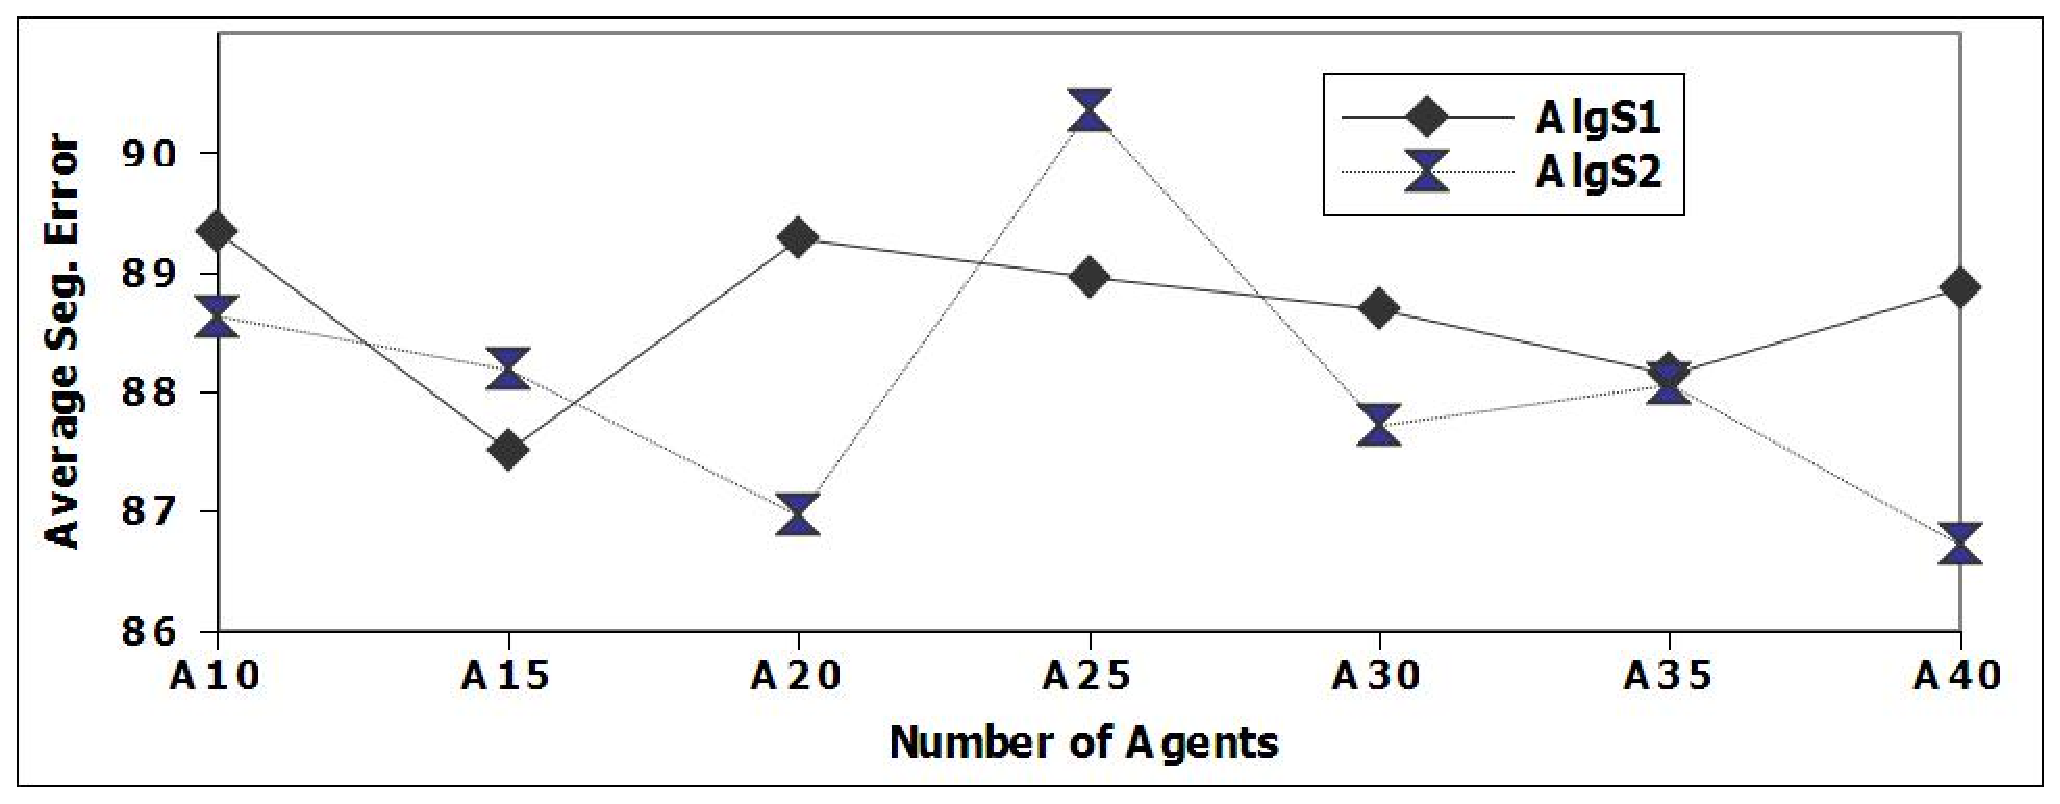
\includegraphics[scale=0.5]{paperImages/swarmAgentTest.jpg.eps}
	 	\caption{Segmentation Error Vs. Number of agents}
	 	\label{fig:swarmtesting}
	%\caption{Experiments results :} a)    b) c) 
\end{figure} 

\begin{figure}
	\centering		
	 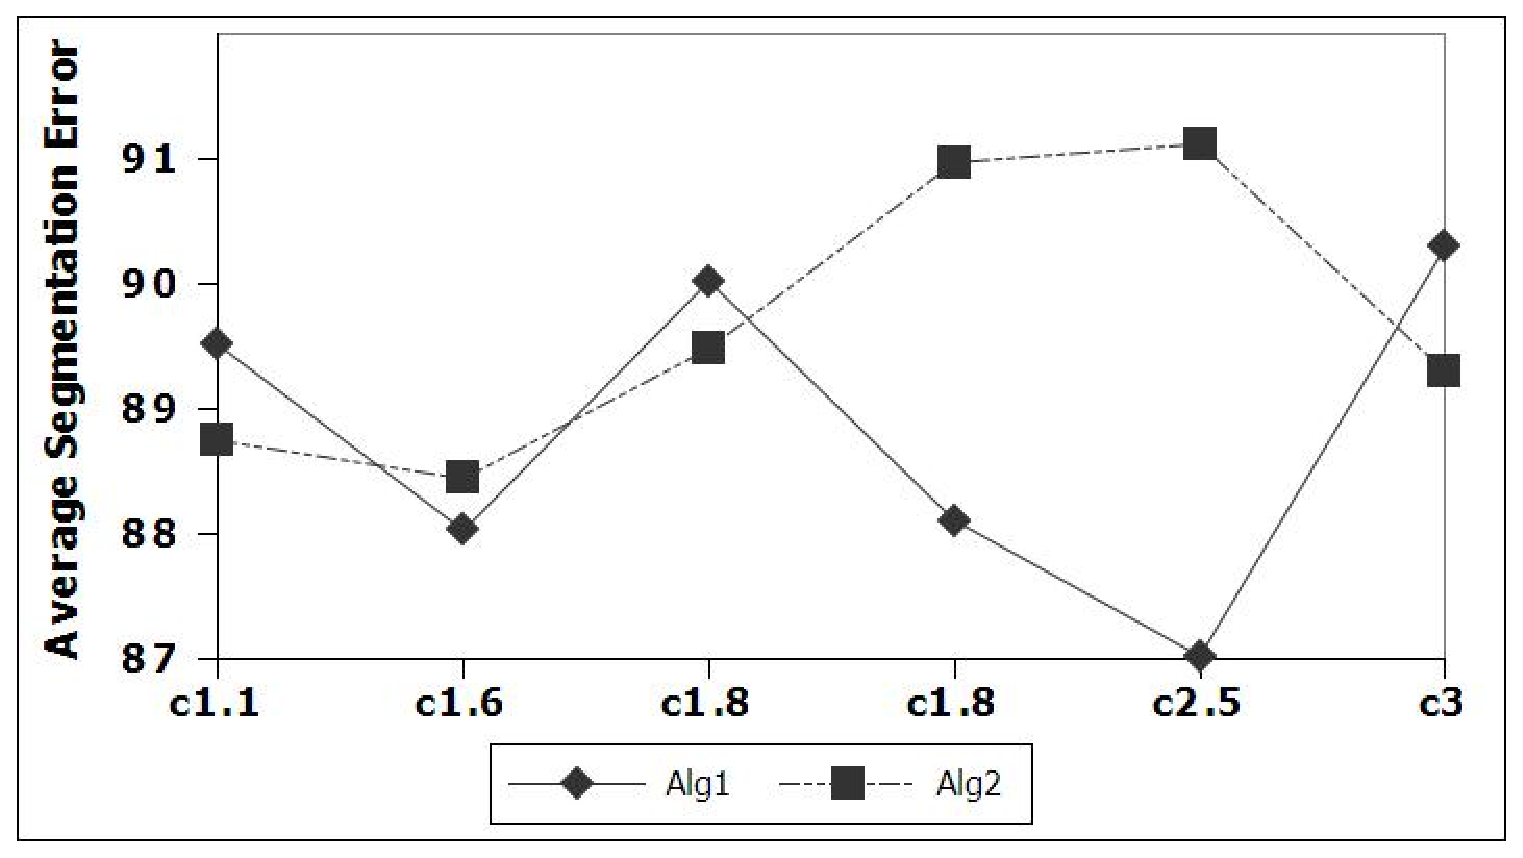
\includegraphics[scale=0.5]{paperImages/swarmParamterC.jpg.eps}
	 	\caption{Segmentation Error Vs. PSO parameters C1}
	 	\label{fig:swarmtesting2}
	%\caption{Experiments results :} a)    b) c) 
	
\end{figure} 


\begin{figure}
	\centering
		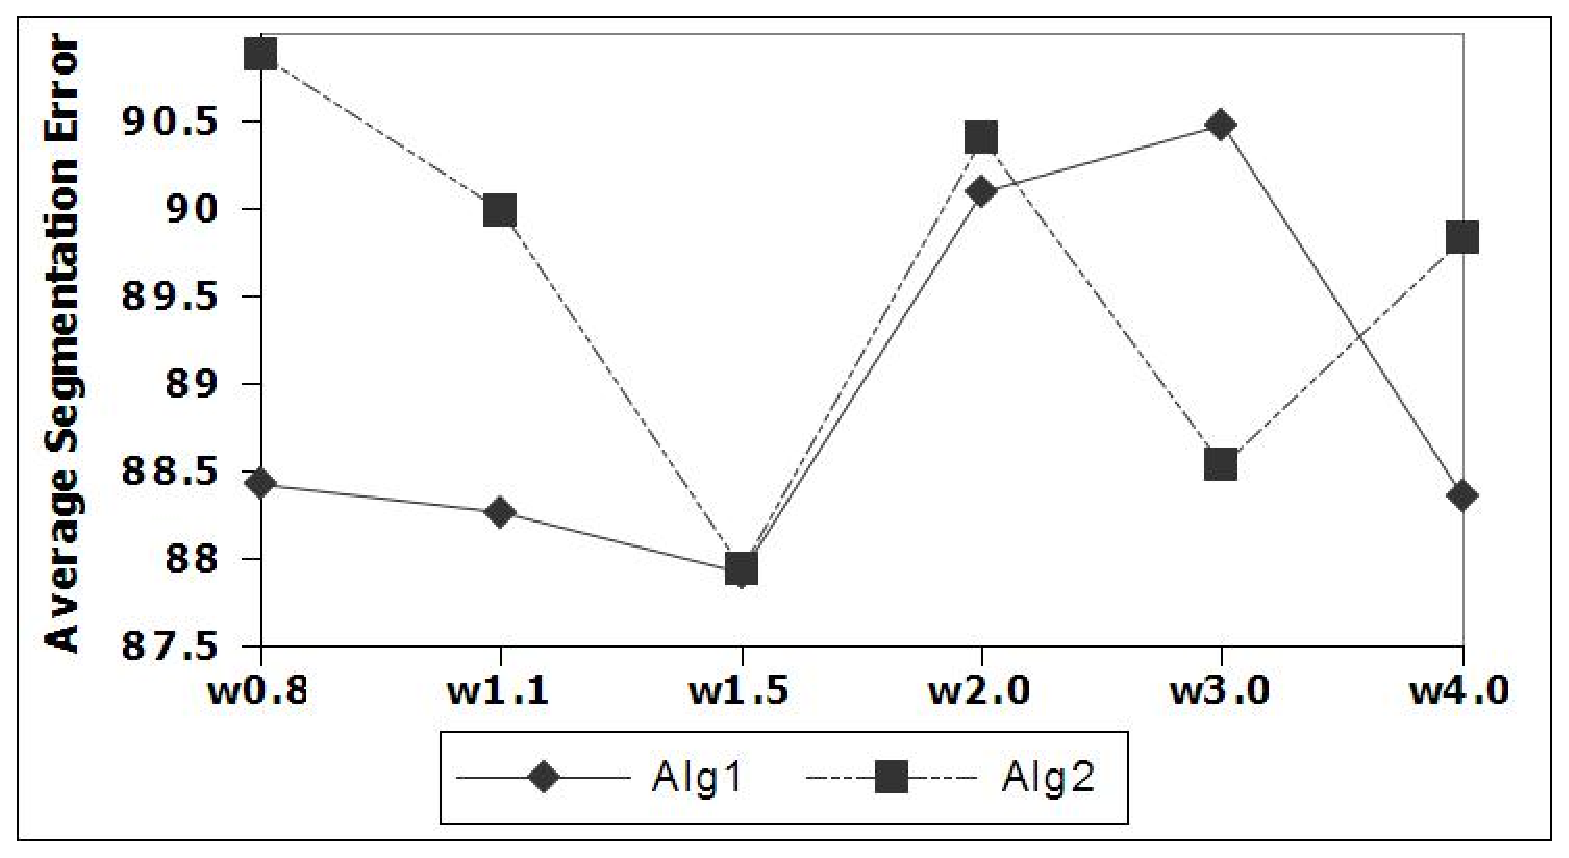
\includegraphics[scale=0.6]{paperImages/swarmparamterw.jpg.eps}
	\caption{Segmentation Error Vs. PSO parameters W.}
	\label{fig:swarmparamterw.jpg}
\end{figure}


%The fig. \ref{fig:dataerrorvsiteration.jpg} display the effect of the size of swarm population on the number of vertex reported while segmenting the stroke.\footnote{The fewer the vertex the better the segmentation} The graphs shows that as the number of iteration increase there is a decrease in error until the error reach a saturation and any increase in number of iteration does not affect the error calculated. Similar behavior is noticed in fig. \ref{fig:datapopulation.jpg}.  These curves and test result in choosing the swarm parameters $c_1,c_2$ and maximum number of iteration and the swarm population. The final values are for maximum number of iteration = 150 with 15 particle for better compensation in the time domain. 

%\begin{figure}
%	\centering
%		\includegraphics[scale=0.8]{images/dataerrorvsiteration.jpg.eps}
%	\caption{Error vs. iterations }
%	\label{fig:dataerrorvsiteration.jpg}
%\end{figure}
%\begin{figure}
%	\centering
%		\includegraphics[scale=0.8]{images/datapopulation.jpg.eps}
%	\caption{Swarm Population }
%	\label{fig:datapopulation.jpg}
%\end{figure}


\subsection{Segmentation Algorithms}
\label{sec:SegmentationAlgorithms}
The result of the segmentation algorithm can be viewed in the Figure \ref{fig:results1}. This result shows the originals stroke and the segmentation that the system generated for the stroke. Figure \ref{fig:results2} shows the result of \textsl{AlgS1} and \textsl{AlgS2} for the same input strokes.  Figure \ref{fig:results3} shows the output of \textsl{Alg3} to the same set of input strokes. It clearly shows that \textsl{AlgS2} have better segmentation results than both \textsl{AlgS1} and \textsl{Alg3} but since these segmentation are subjective to what the user intended to draw the next section will focus on the evaluating the segmentation algorithms using the effect on the recognition accuracy. 

\begin{figure}

	\centering
				\subfigure{\includegraphics[scale=0.45]{results/result1.eps}}
					\subfigure{	\includegraphics[scale=0.6]{results/result1logic.eps}}
	\caption{Segmentation Results of \textsl{AlgS1}}
	\label{fig:results1}

\end{figure}

\begin{figure}
	\centering
			\subfigure{	\includegraphics[scale=0.45]{results/result2.eps}}
			\includegraphics[scale=0.6]{results/result2logic.eps}
	\caption{Segmentation Results of \textsl{AlgS2}}
	\label{fig:results2}
\end{figure}
\begin{figure}
	\centering
		\subfigure{
		\includegraphics[scale=0.45]{results/result3.eps}}
			\subfigure{\includegraphics[scale=0.55]{results/result3logic.eps}}
		
	\caption{Segmentation Results of \textsl{Alg3} }
	\label{fig:results3}
\end{figure}



\subsection {Recognition system}
\label{sec:RecognitionAlgorithms}

several experiments is presented to test the different segmentation algorithms on the three data set used in our system. Algorithms (\textsl{AlgS1}, \textsl{AlgS2} and \textsl{Alg3} (in section \ref{sec:BenchMarckAlgorithm})) were tested individually with and without the ellipse fitting module. The final system (Choosing the Minimum error of (\textsl{AlgS1}, \textsl{AlgS2}) was evaluated on the three dataset(HS, EL and LD datasets ). Figure \ref{fig:test1},\ref{fig:testEL} and \ref{fig:testLD} shows the accuracy achieved by each algorithm. Theses experiments were done using the whole dataset as 75\% of the data as test set and 25\% as training. The results shows that \textsl{AlgS2} with the ellipse fitting module gives better recognition rate across all datasets (Figure \ref{fig:test1},\ref{fig:testEL} and \ref{fig:testLD} ). Even though, \textsl{AlgS1} gives better result than \textsl{Alg3} in both EL-DB and HS-DB it perform poorly in LD-DB due to the high number of curves in every symbol in this dataset. These result are proved using different number of samples per category as shown in Figures \ref{fig:LDRes}, \ref{fig:ElRes}. 
% i need to organize this as following. 
% number 1. differnt algorithm on different data 
% which algortihm is better oon which data 
% on ld and el  the alg2  is better, 

%We performed several experiments to evaluate the presented recognition system. Firstly we tested recognition accuracy of shapes in the data set with both algorithms (\textsl{AlgS1} and \textsl{AlgS2}). We also implemented the segmentation algorithm described in \cite{earlyprocess} (\textsl{Alg3} in section \ref{sec:BenchMarckAlgorithm} )  to use as reference to compare it with our swarm algorithms. Figure \ref{fig:test1},\ref{fig:testEL} and \ref{fig:testLD}  shows the accuracy achieved by each algorithm. The two swarm algorithms were tested with and without the ellipse fitting module. The ellipse fitting module appears to be superior. The result shows that combining both algorithms (\textsl{AlgS1} and \textsl{AlgS2}) outperform any single algorithm. %show that combining algorithms achieve higher accuracy than any single algoirthm. 
%improves the results.% with both the \textit{DPSO} algorithms.% The results show that both \textit{DPSO} algorithms achieve better result than other algorithms. 
\begin{figure}
	\centering		
	 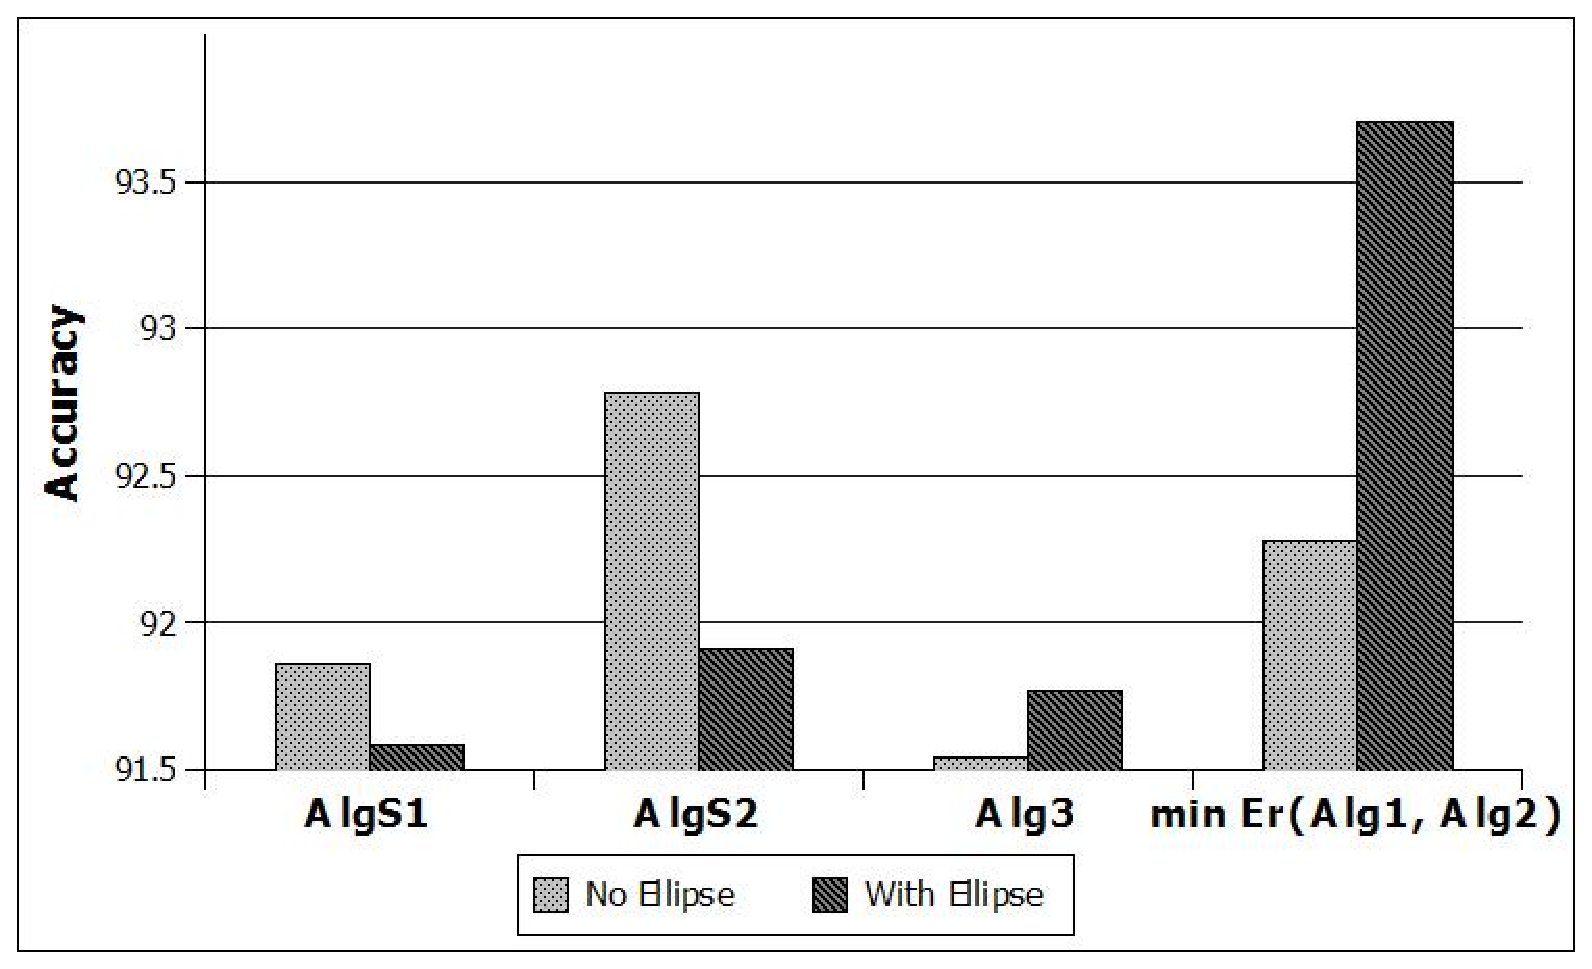
\includegraphics[scale=0.4]{paperImages/testAlg.jpg.eps}
	 	\caption{Algorithm comparison on HS-DB} The recognition rate of different algorithms. 
	 	\label{fig:test1}
	%\caption{Experiments results :} a)    b) c) 
\end{figure} 
\begin{figure}
	\centering		
	 \includegraphics[scale=0.8]{results/AlgLD.eps}
	 	\caption{Algorithm comparison on LD-DB} The recognition rate of different algorithms. 
	 	\label{fig:testLD}
	%\caption{Experiments results :} a)    b) c) 
\end{figure} 

\begin{figure}
	\centering		
	 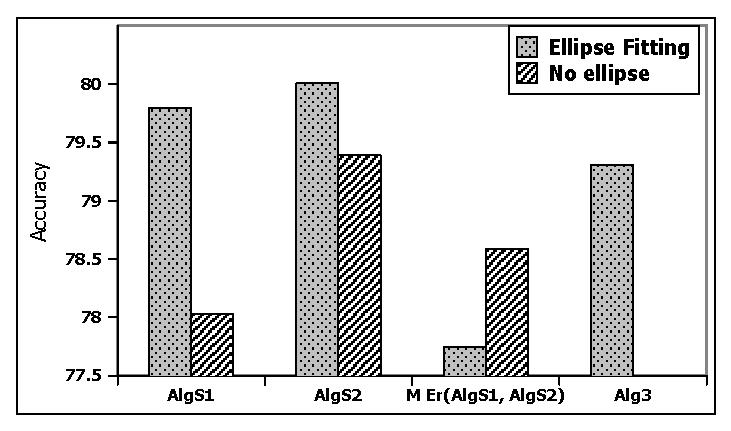
\includegraphics[scale=0.8]{results/AlgEL.eps}
	 	\caption{Algorithm comparison on EL-DB} The recognition rate of different algorithms. 
	 	\label{fig:testEL}
	%\caption{Experiments results :} a)    b) c) 
\end{figure} 

 
 
 
 
\begin{figure}
	\centering
		\includegraphics[scale=0.6]{results/LDRes.eps}
	\caption{Result Algorithms on LD-DB}
	\label{fig:LDRes}
	
	
\end{figure}
\begin{figure}
	\centering
		\includegraphics[scale=0.6]{results/ElRes.eps}
	\caption{Results of Algorithms on EL-DB}
	\label{fig:ElRes}
\end{figure}


 

\subsubsection {Evaluating Different Datasets}
 \label{sec:EffectsofSymbolComplixity}
 
 The effects of symbol complexity in a dataset were testing in the following experiment. These experiments test how many samples will be required to finally obtain good performance from the recognizer system. In the following experiments, we tested the system using different number of sample per category. 
 Figure \ref{fig:Alg1Ds} and \ref{fig:Alg2Ds} shows that Hs-DB requires more number of sample for training to achieve same result as in other data sets. This is due that it contains less signal and conceptual variation that the other two datasets. Figure \ref{fig:samplesofHS-DB.jpg} shows sample of data collected from one user in Hs-Db it is clear that it has reasonable amount of variation between users but it is limited. Recognizing symbols that contains high variation in drawing style using fewer symbols in training prove the efficiency of our system.
 \begin{figure}
	\centering
		\includegraphics{results/Alg1Ds.eps}
	\caption{AlgS1 on different datasets}
	\label{fig:Alg1Ds}
\end{figure}
\begin{figure}
	\centering
		\includegraphics{results/Alg2Ds.eps}
	\caption{AlgS2 on different Datasets }
	\label{fig:Alg2Ds}
\end{figure}
 
  Figure \ref{} and \ref{} shows examples of correctly recognized symbol using our system. The figure shows that system recognized some hard to recognize example in both EL-DB and DL-DB. An example of symbols that was not correctly recognized are in Figure \ref{}. Most of the wrong classifications were due to how messy the user draw symbols and how similarly they are conceptual. Table \ref{} show the confusion matrix of EL-DB which shows that most error were between capacitor, batter and crystal which differ only on number of parallel lines. Table \ref{tab:ConfusionMatrix} (confusion matrix) shows the types of error in Hs-DB which shows that the system was confused between parallelogram and trapezoid, moon and arch. Those errors were due to users drawing styles as some user may draw a parallelogram as a trapezoid. 

\begin{figure}
	\centering
	\includegraphics[scale=0.5]{results/samplesofHS-DB.jpg.eps}
	\caption{Hs-DB shapes drawn by single user}
	\label{fig:samplesofHS-DB.jpg}
\end{figure}
 \begin{table*}
	\centering
	%\small
%	\scalebox{0.7}{
		%	\begin{tabular}{|c|c|c|c|c|c|c|c|c|c|c|c|c|c|}\hline 
	\scalebox{0.7}{
		\begin{tabular}{|c|c|c|c|c|c|c|c|c|c|c|c|c|c|}\hline 
 Categories 	&ellipse	&heart	&trapezoid	&pentagon	&arch	&hexagon	&square	&triangle	&cube	&cylinder	&parallelogram	&moon	&callout\\ \hline
ellipse	&155	&9	&0	&0	&0	&5	&0	&0	&0	&0	&0	&6	&0\\ \hline
heart	&0	&109	&1	&1	&25	&0	&0	&1	&0	&0	&2	&1	&1\\ \hline
trapezoid	&0	&0	&103	&5	&2	&0	&0	&2	&0	&0	&34	&0	&0\\ \hline
pentagon	&0	&0	&20	&121	&0	&20	&6	&2	&0	&0	&1	&0	&0\\ \hline
arch	&0	&1	&13	&0	&86	&0	&0	&2	&3	&0	&2	&0	&0\\ \hline
hexagon	&0	&0	&0	&0	&0	&98	&0	&0	&0	&0	&0	&0	&0\\ \hline
square	&0	&0	&1	&0	&2	&0	&107	&14	&0	&0	&8	&1	&0\\ \hline
triangle	&0	&0	&7	&0	&1	&0	&0	&89	&0	&0	&12	&4	&0\\ \hline
cube	&0	&0	&0	&0	&0	&0	&0	&0	&147	&0	&0	&0	&0\\ \hline
cylinder	&0	&0	&0	&6	&2	&8	&16	&0	&4	&156	&1	&10	&0\\ \hline
parallelogram	&0	&0	&4	&0	&0	&0	&0	&0	&0	&0	&91	&0	&0\\ \hline
moon	&0	&3	&3	&2	&17	&0	&9	&17	&0	&0	&2	&133	&11\\ \hline
callout	&1	&34	&0	&22	&21	&22	&16	&25	&0	&0	&0	&0	&143\\ \hline
		\end{tabular}
			}
 		%\end{tabular}
 	%}
	\caption{Confusion Matrix}
	\label{tab:ConfusionMatrix}
	%\end{minipage}
\end{table*}

%\begin{figure}
%	\centering
%		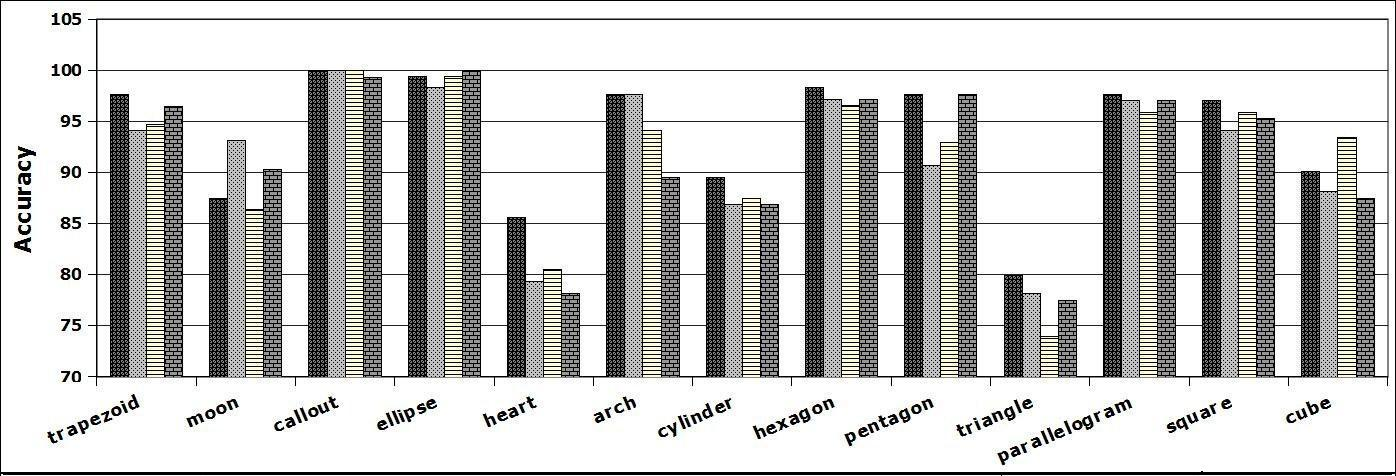
\includegraphics[scale=0.5]{results/testsym.eps}
%	\caption{Symbols Comparison} The effect of symbol complexity.  %The graph shows the recognition rate of each symbol using different algorithms. 
%	\label{fig:test2}
%\end{figure}  

Another experiment we implemented was to investigate the effect of symbol complexity and type on the recognition rate. Figure \ref{fig:test2} shows the achieved accuracy of each symbol by our algorithms compared to \cite{earlyprocess} (\textsl{Alg3}). It is clearly noted that symbols that have only line segments achieve higher accuracy rate than other symbols.  The results indicate that algorithm \textsl{AlgS1} achieve better performance than algorithm \textsl{AlgS2} in the symbols that consist only of lines. This is understandable because algorithm \textsl{AlgS1} divides strokes into line segments only but \textsl{AlgS2} is able to divide strokes into lines and curves based on the minimum error of the segment itself. Algorithm \textsl{Alg3} gives good performance as long as the symbols consist of combination of lines and curves, if the stroke consists of only curve or lines the algorithm may lead to wrong segmentation result. This is because the system divides the stroke first to line segments then tries to decide if each segment can be represent better as a curve unlike algorithm \textsl{AlgS2} where the curve segments are tested while choosing the best segmentation. Combining both algorithm \textsl{AlgS1} and \textsl{AlgS2} improved the recognition rate of all symbols. The penalty for this improved performance is the computational time required to run both swarm algorithms. Table \ref{tab:ConfusionMatrix} shows the confusion matrix of symbols. The table shows that errors are only between two sets of symbols moon with triangles and trapezoid with triangles. This observation is understandable as the symbols are visually similar but the system must be able to differentiate between them. This led us to the next experiment to choose best set of feature to recognize symbols. 
 
 \begin{figure}
	\centering
		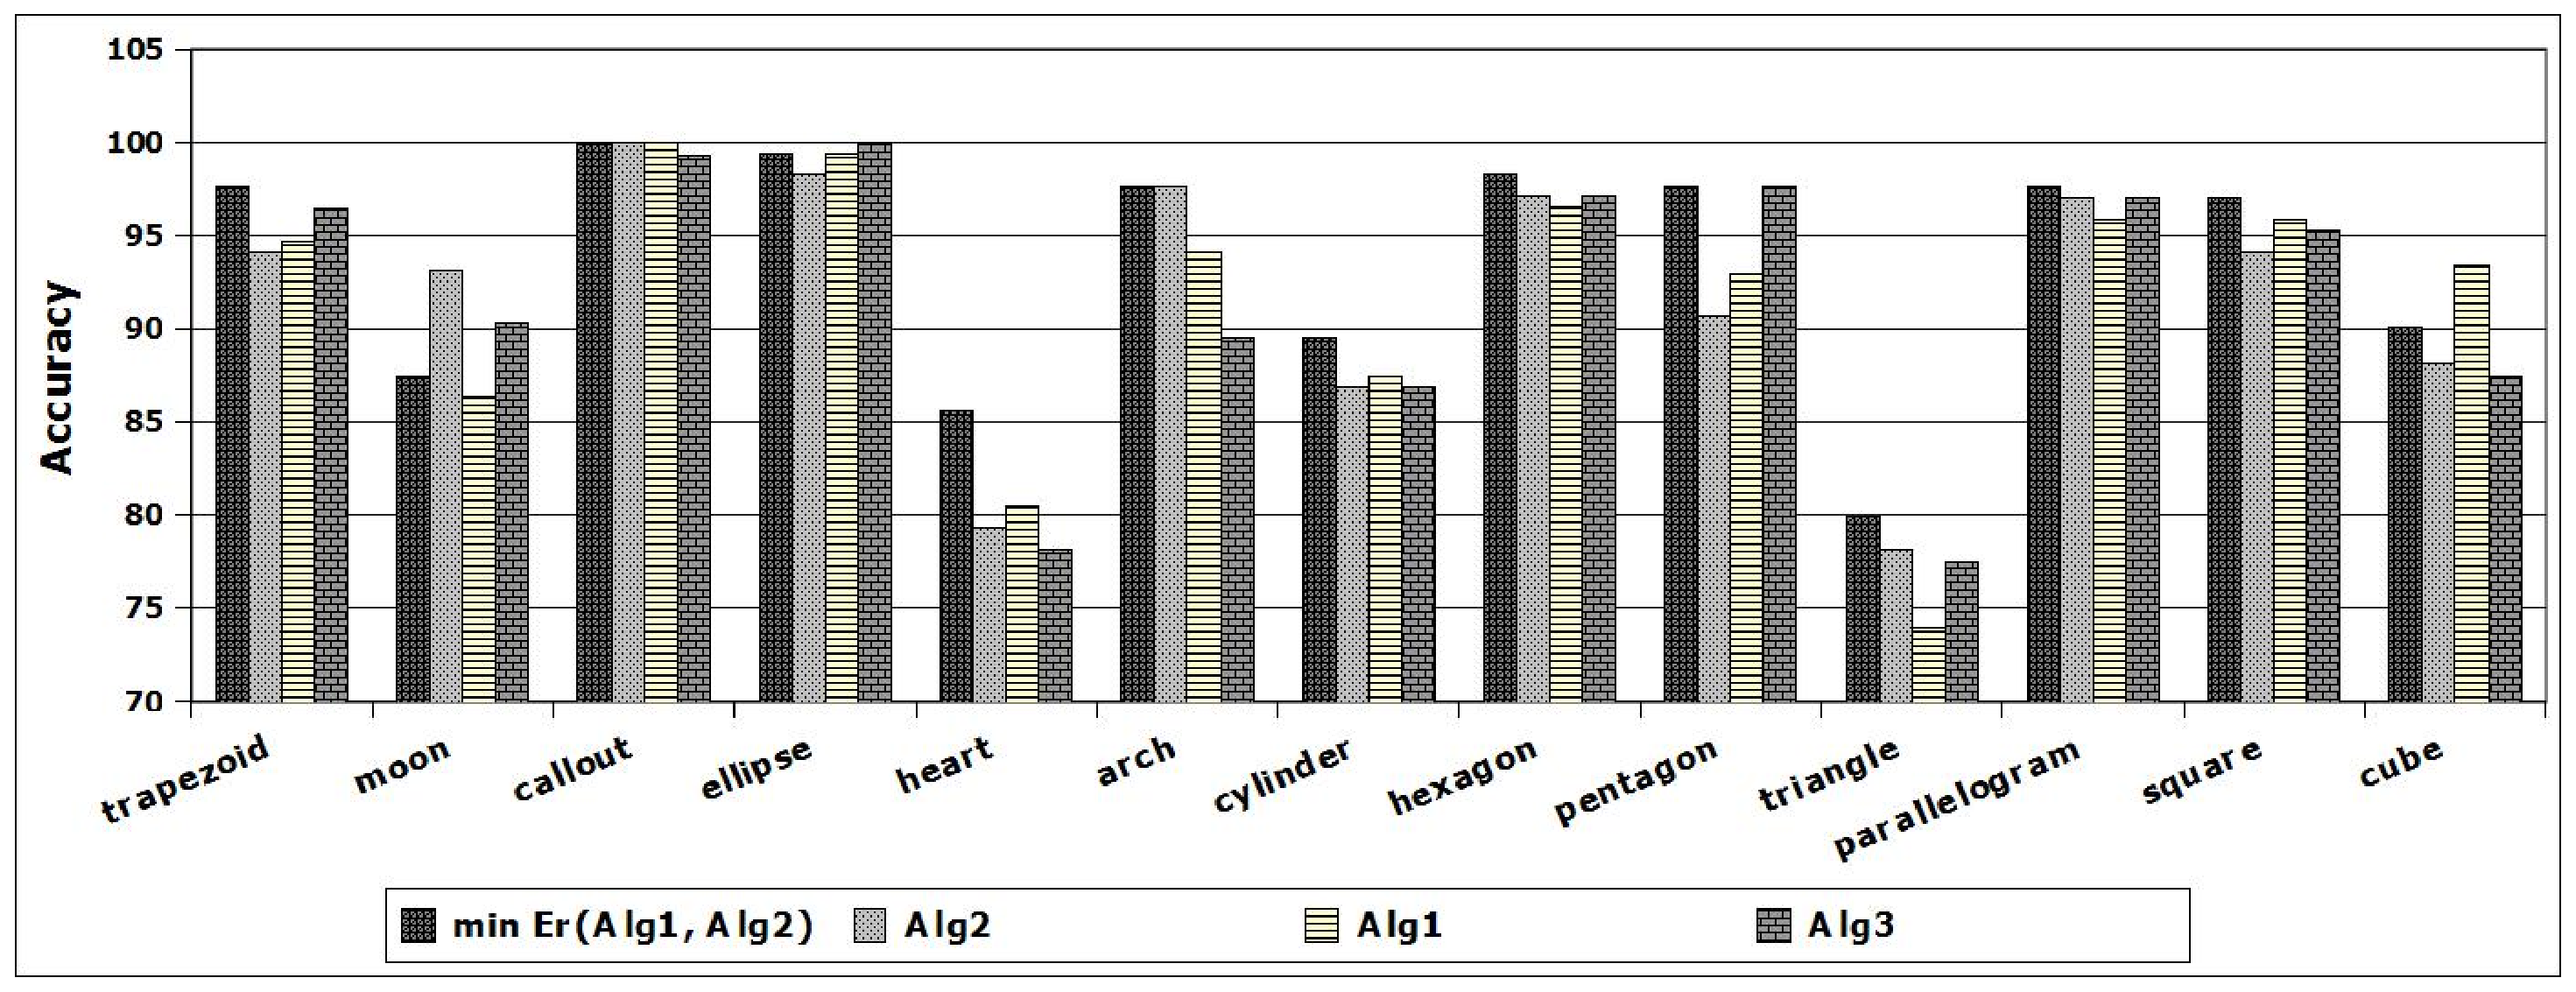
\includegraphics[scale=0.35]{paperImages/testsym.jpg.eps}
	\caption{Symbols Comparison on HS-DB} The effect of symbol complexity.  %The graph shows the recognition rate of each symbol using different algorithms. 
	\label{fig:test2}
\end{figure}  

\begin{figure}
	\centering
		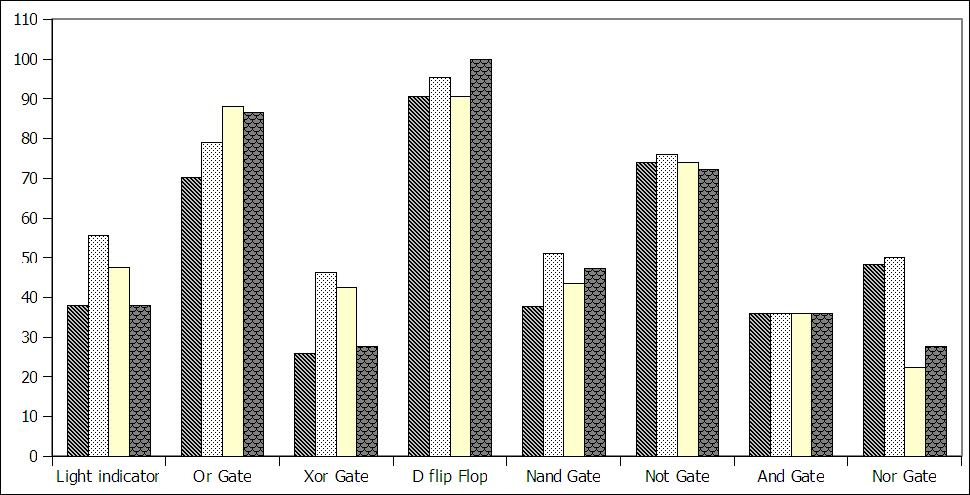
\includegraphics[scale=0.5]{paperImages/LDsymbols.jpg.eps}
	\caption{Symbols Comparison on LD-DB symbols}.  %The graph shows the recognition rate of each symbol using different algorithms. 
	\label{fig:LDtest2}
\end{figure}  


\begin{figure}
	\centering
		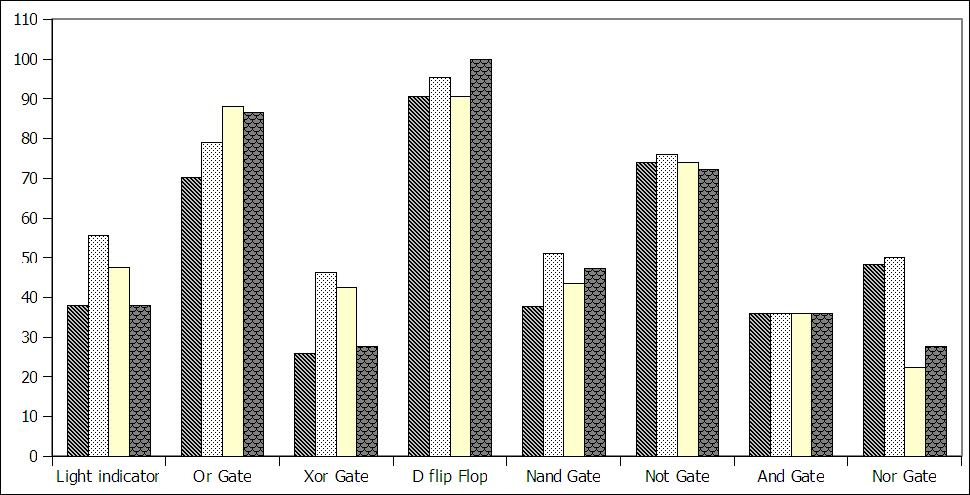
\includegraphics[scale=0.1]{paperImages/LDsymbols.jpg.eps}
	\caption{Symbols Comparison on EL-DB symbols}.  %The graph shows the recognition rate of each symbol using different algorithms. 
	\label{fig:ELtest2}
\end{figure}  
 
 
\subsubsection{Features Comparisons}
\label{sec:featuresComparisions}
Different feature sets are tested to determine the best features that can used in sketch and symbol recognition. Figure\ref{fig:testFeaturesAllHS} shows the result of different feature sets from the basic four sets (\textbf{FS1,FS2,FS3,FS4}). Result shows that (\textbf{FS2}) Rubine features \cite{gestureexample12} gives the worst results when used alone without any other features. This is because they are mainly computed for single stroke gestures and fare bad in multi-stroke symbols \cite{compareFeaturSVM}. Features \textbf{(FS4)} gives good results but it is improved by adding structural features \textbf{(FS1)}.  Figure \ref{fig:testFeaturesAllMD} shows the similar results on \textsl{EL-DB} and \textsl{LD-DB} dataset. The figures show that on both datasets \textbf{FS1} perform better than on \textsl{HS-DB}, this is a result that shapes in the \textsl{EL-DB} and \textsl{LD-DB} has more structural and conceptual differences than shapes in \textsl{HS-DB}. In \cite{HeloiseBeautification} used Zernike moment (FS3) and mentioned that order higher than 8 yield to little or no improvement. In our system we used much higher order to reach this saturation level. This is due to the level of details in the EL-DB and DL-DB sets. % achieved  HS-DB a
 \begin{figure}
	\centering
		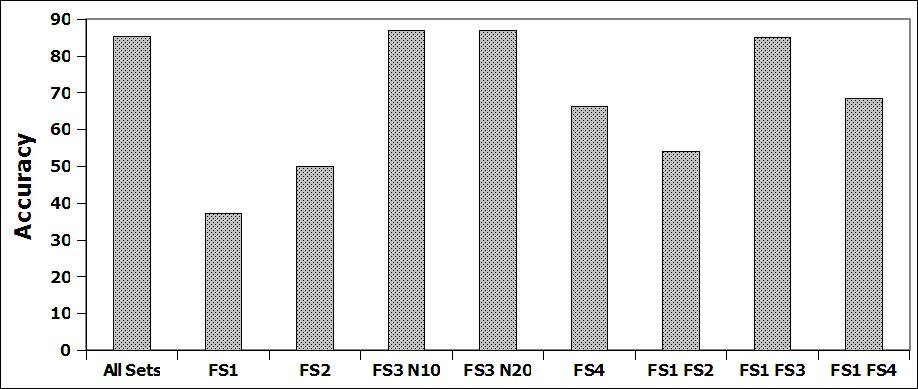
\includegraphics[scale=0.5]{paperImages/featuresdifference.jpg.eps}
	\caption{Feature Comparison on Hs-DB} The effect of different features on accuracy.  %The graph shows the recognition rate of each symbol using different algorithms. 
	\label{fig:testFeaturesAll}
\end{figure}  


 \begin{figure}
	\centering
		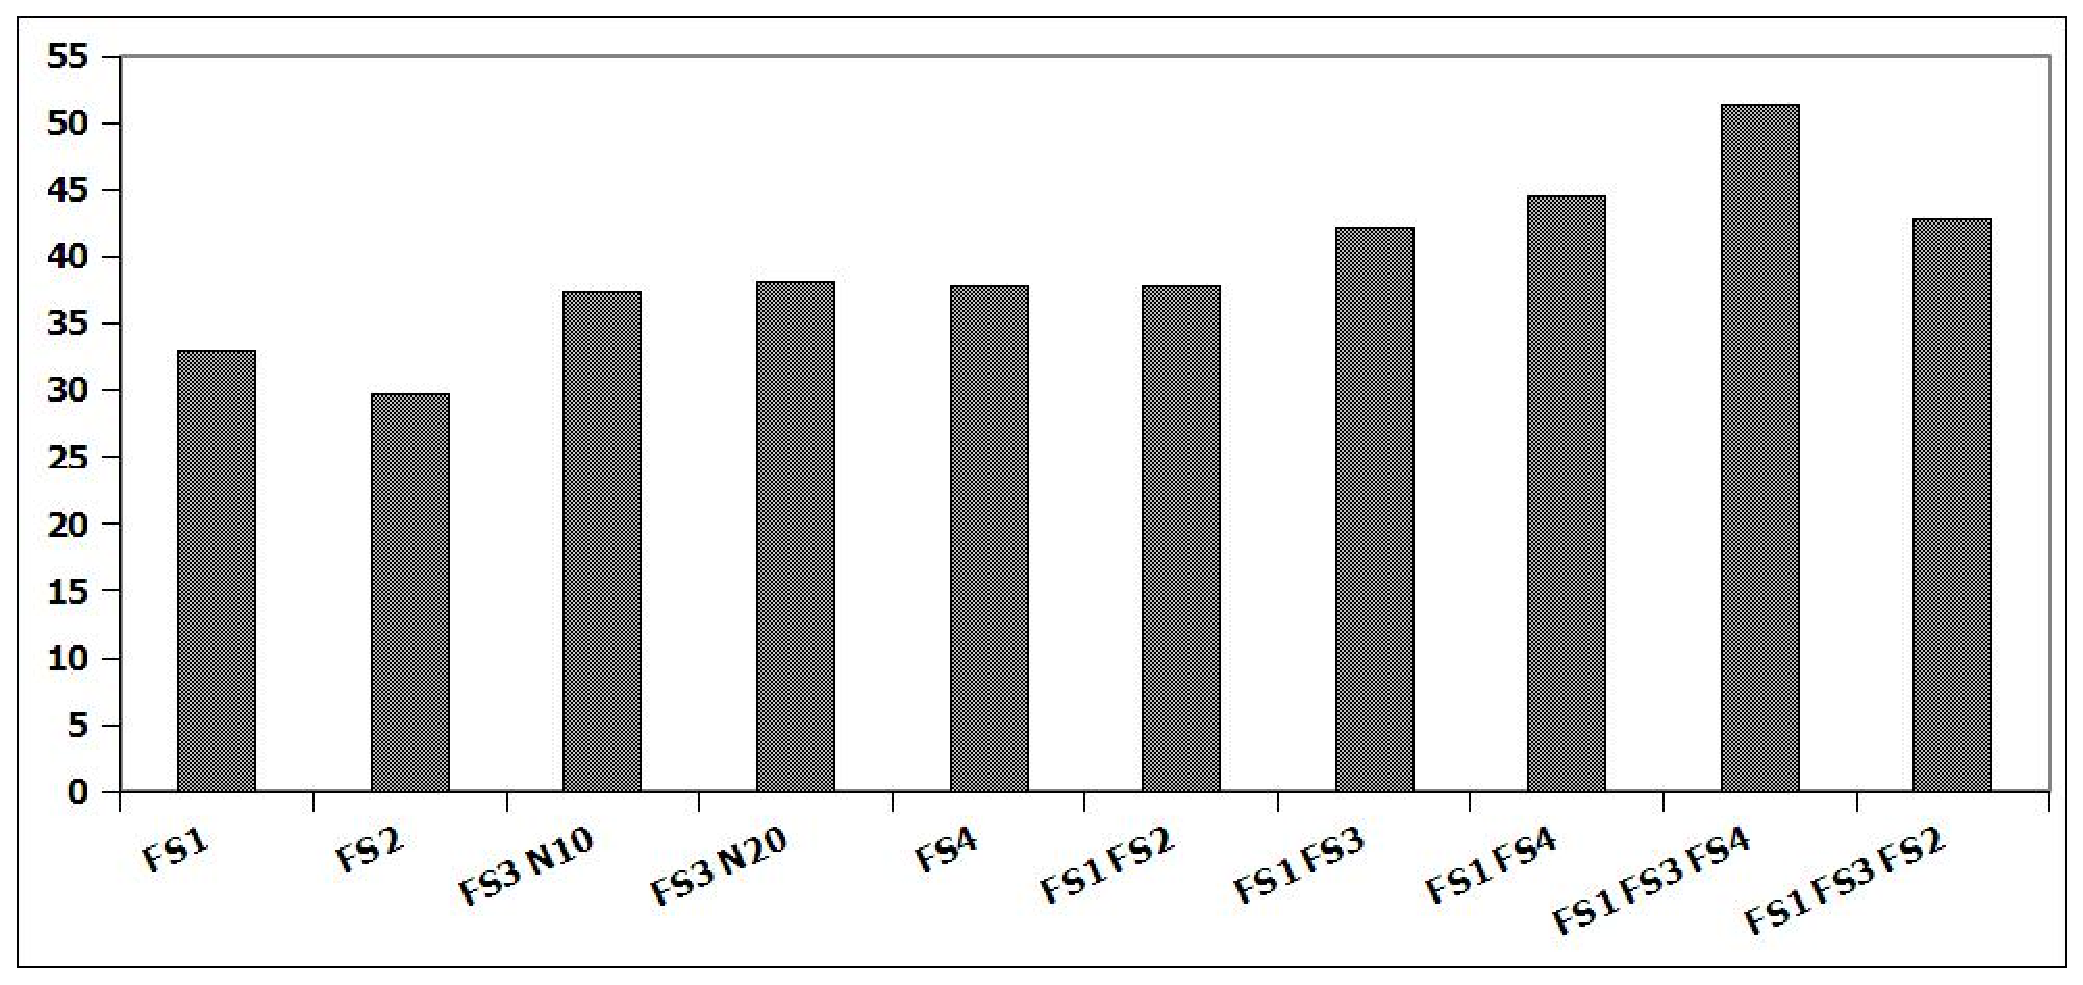
\includegraphics[scale=0.5]{paperImages/featuresLD.jpg.eps}
	\caption{Feature Comparison on LD-DB} The effect of different features on accuracy.  %The graph shows the recognition rate of each symbol using different algorithms. 
	\label{fig:testFeaturesAll}
\end{figure}  

 \begin{figure}
	\centering
		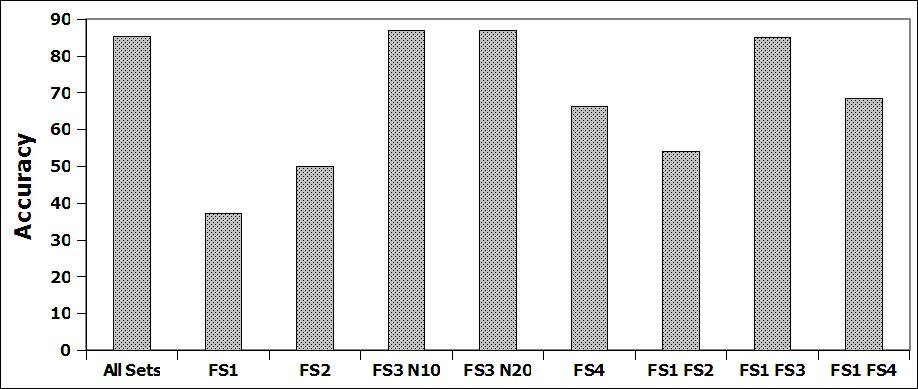
\includegraphics[scale=0.5]{paperImages/featuresdifference.jpg.eps}
	\caption{Feature Comparison on EL-DB} The effect of different features on accuracy.  %The graph shows the recognition rate of each symbol using different algorithms. 
	\label{fig:testFeaturesAll}
\end{figure}  


 The main features affected by the segmentation stage are the geometric features computed in\textbf{FS1}. Hence those are the features we used to estimate the efficiency of the segmentation algorithm. The recognition accuracy using only the geometrical features is reported in Figure \ref{fig:testFeatonly} . The figure shows that \textsl{AlgS2} achieve better results.  %effect of the segmentation algorithm 
 %Figure \ref{fig:SampleSeg} shows a sample of the output of the segmentation block. The result of segmentation block is tested by their effect on the final recognition results using the features that will be highly affected using different algorithms like \textbf{FS1} and \textbf{FS4} (Section\ref{sec:Recognition}). Figure \ref{fig:testFeatonly} shows the result of the different algorithms using only \textbf{FS1 }features. 
 \begin{figure}
	\centering
		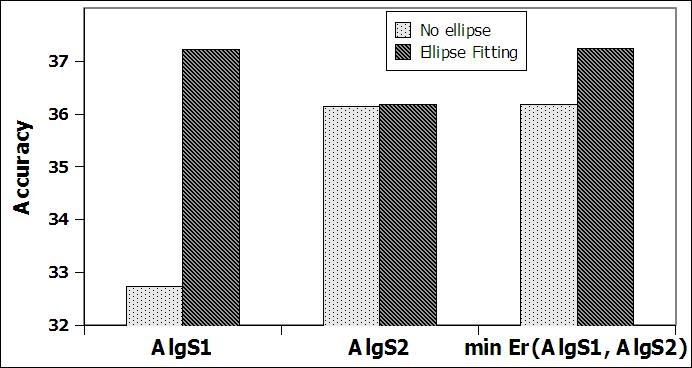
\includegraphics[scale=0.4]{paperImages/featureFS1only.jpg.eps}
	\caption{The effect of segmentation on Hs-DB accuracy} %The effect of symbol complexity.  %The graph shows the recognition rate of each symbol using different algorithms. 
	\label{fig:testFeatonly}
\end{figure}  
 \begin{figure}
	\centering
		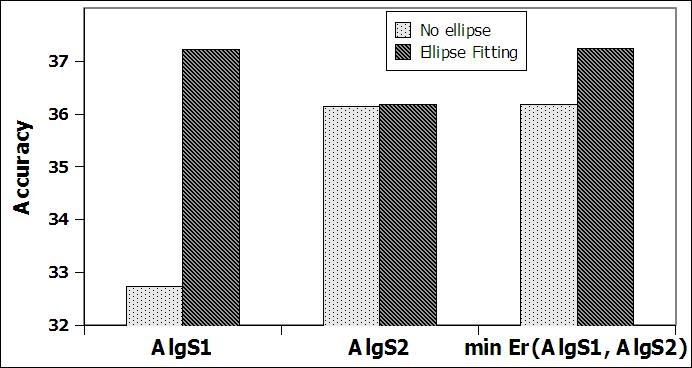
\includegraphics[scale=0.4]{paperImages/featureFS1only.jpg.eps}
	\caption{The effect of segmentation on LD-DB accuracy} %The effect of symbol complexity.  %The graph shows the recognition rate of each symbol using different algorithms. 
	\label{fig:LDtestFeatonly}
\end{figure}  
 \begin{figure}
	\centering
		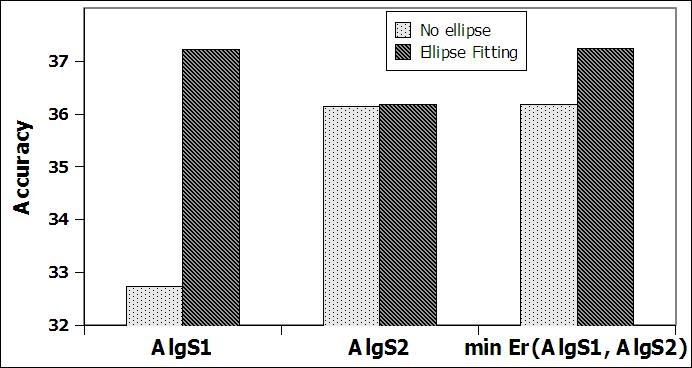
\includegraphics[scale=0.4]{paperImages/featureFS1only.jpg.eps}
	\caption{The effect of segmentation on EL-DB accuracy} %The effect of symbol complexity.  %The graph shows the recognition rate of each symbol using different algorithms. 
	\label{fig:ELtestFeatonly}
\end{figure}  
%
% \begin{figure}
%	\centering
%		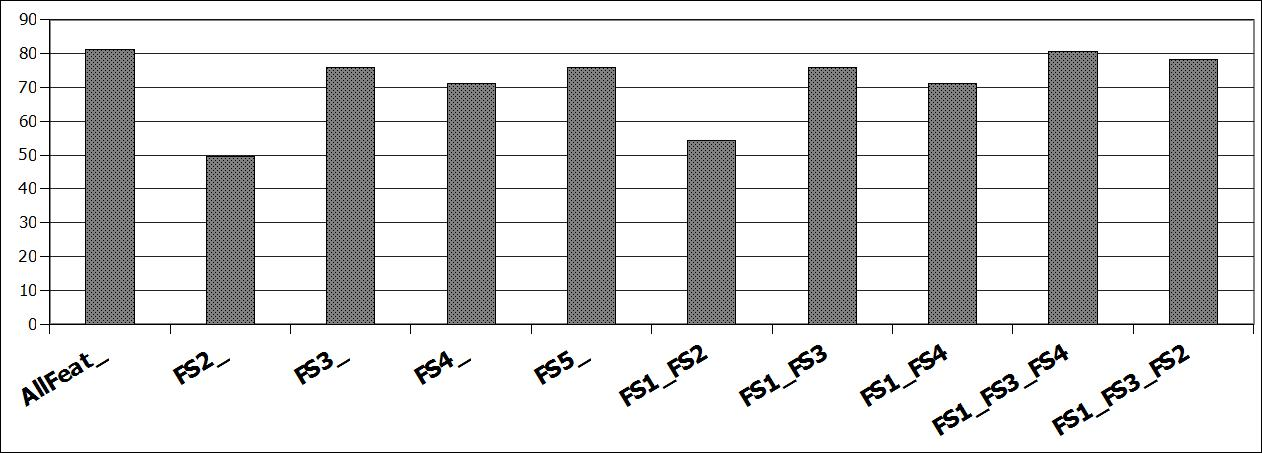
\includegraphics[scale=0.5]{results/testFeat.eps}
%	\caption{Feature Comparison} The effect of different features on accuracy on \textsl{Hs-DB}.  %The graph shows the recognition rate of each symbol using different algorithms. 
%	\label{fig:testFeaturesAllHS}
%\end{figure}  
%
% \begin{figure}
%	\centering
%		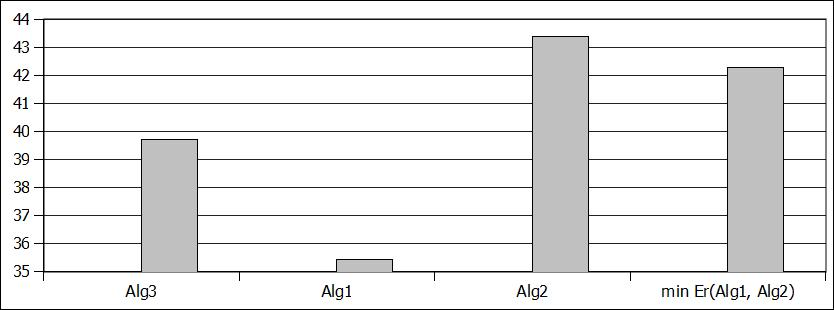
\includegraphics[scale=0.5]{results/testF1.eps}
%	\caption{Feature Comparison} The effect of different features on accuracy on \textsl{MD-DB}.  %The graph shows the recognition rate of each symbol using different algorithms. 
%	\label{fig:testFeaturesAllMD}
%\end{figure}  


\section{Summary}
\label{sec:ResultSummary}

The result illustrated in this chapter shows the work done on the system and experiments performed. We showed result of three different dataset. The system performed better than most known algorithm on the EL-DB and LD-DB. This is due to the focus on structure and stroke based properties gained from the system after correctly segmenting the input strokes. The result also showed that even using \textsl{AlgS2} only as the segmentation algorithm the system perform better than other segmentation algorithm. Using different databases shows that the more the structure differences in the symbols the better recognition rate. LD-DB proved to have the lowest recognition rate due to the high similarity between its symbols.    % better than 

%\section{ BenchMark Results }
%\label{sec:BenchMarkResults}

